\documentclass[12pt,a4paper]{article}
\usepackage{amsmath,amscd,amsbsy,amssymb,latexsym,url,bm,amsthm}
\usepackage{epsfig,graphicx,subfigure}
\usepackage{enumitem,balance}
\usepackage{wrapfig}
\usepackage{mathrsfs,euscript}
\usepackage[usenames]{xcolor}
\usepackage{hyperref}
\usepackage[vlined,ruled,linesnumbered]{algorithm2e}
\usepackage{float}
\usepackage{array}
\hypersetup{colorlinks=true,linkcolor=black}

\newtheorem{theorem}{Theorem}
\newtheorem{lemma}[theorem]{Lemma}
\newtheorem{proposition}[theorem]{Proposition}
\newtheorem{corollary}[theorem]{Corollary}
\newtheorem{exercise}{Exercise}
\newtheorem*{solution}{Solution}
\newtheorem{definition}{Definition}
\theoremstyle{definition}

\renewcommand{\thefootnote}{\fnsymbol{footnote}}

\newcommand{\postscript}[2]
{\setlength{\epsfxsize}{#2\hsize}
	\centerline{\epsfbox{#1}}}

\renewcommand{\baselinestretch}{1.0}

\setlength{\oddsidemargin}{-0.365in}
\setlength{\evensidemargin}{-0.365in}
\setlength{\topmargin}{-0.3in}
\setlength{\headheight}{0in}
\setlength{\headsep}{0in}
\setlength{\textheight}{10.1in}
\setlength{\textwidth}{7in}
\makeatletter \renewenvironment{proof}[1][Proof] {\par\pushQED{\qed}\normalfont\topsep6\p@\@plus6\p@\relax\trivlist\item[\hskip\labelsep\bfseries#1\@addpunct{.}]\ignorespaces}{\popQED\endtrivlist\@endpefalse} \makeatother
\makeatletter
\renewenvironment{solution}[1][Solution] {\par\pushQED{\qed}\normalfont\topsep6\p@\@plus6\p@\relax\trivlist\item[\hskip\labelsep\bfseries#1\@addpunct{.}]\ignorespaces}{\popQED\endtrivlist\@endpefalse} \makeatother

\begin{document}
	\noindent
	
	%========================================================================
	\noindent\framebox[\linewidth]{\shortstack[c]{
			\Large{\textbf{Lab05-DynamicProgramming}}\vspace{1mm}\\
			CS214-Algorithm and Complexity, Xiaofeng Gao, Spring 2021.}}
	\begin{center}
		\footnotesize{\color{red}$*$ If there is any problem, please contact TA Haolin Zhou.}
		
		% Please write down your name, student id and email.
		\footnotesize{\color{blue}$*$ Name: Wendi Chen  \quad Student ID: 519021910071 \quad Email: chenwendi-andy@sjtu.edu.cn}
		
	\end{center}
	
	\begin{enumerate}
		\item \textit{Optimal Binary Search Tree.} Given a sorted sequence $K=\left \langle k_{1}, k_{2}, \ldots, k_{n} \right \rangle$ of $n$ distinct keys, and we wish to build a binary search tree from these keys. For each key $k_{i}$, we have a probability $p_{i}$ that a search will be for $k_{i}$. Some searches may be for values not in $K,$ and so we also have $n+1$ \emph{dummy keys} $d_{0}, d_{1}, d_{2}, \ldots, d_{n}$ representing values not in $K$. In particular, $d_{0}$ represents all values less than $k_{1}$, and $d_{n}$ represents all values greater than $k_{n}$. For $i=1,2, \ldots, n-1,$ the dummy key $d_{i}$ represents all values between $k_{i}$ and $k_{i+1}$. For each dummy key $d_{i}$, we have a probability $q_{i}$ that a search will correspond to $d_{i}$. Each key $k_{i}$ is an internal node, and each dummy key $d_{i}$ is a leaf. Every search is either successful (finding some key $k_{i}$ ) or unsuccessful (finding some dummy key $d_{i}$ ), and so we have $ \sum_{i=1}^{n} p_{i}+\sum_{i=0}^{n} q_{i}=1 $. 
		\begin{enumerate}
			\item Prove that if an optimal binary search tree $T$ ($ T $ has the smallest expected search cost) has a subtree $T^{\prime}$ containing keys $k_{i}, \ldots, k_{j},$ then this subtree $T^{\prime}$ must be optimal as well for the subproblem with keys $k_{i}, \ldots, k_{j}$ and dummy keys $d_{i-1}, \ldots, d_{j}$. 
			\item We define $e[i, j]$ as the expected cost of searching an optimal binary search tree containing the keys $k_{i}, \ldots, k_{j} .$ Our goal is to compute $e[1, n]$. Write the state transition equation and pseudocode using \textbf{dynamic programming} to find
			the minimum expected cost of a search in a given binary tree. (\textbf{Remark}: You may use $ w(i, j)=\sum_{l=i}^{j} p_{l}+\sum_{l=i-1}^{j} q_{l} $).
			\item Implement your proposed algorithm in C/C++ and analyze the time complexity. ({\color{blue}The framework Code-OBST.cpp is attached on the course webpage}). Give the minimum search cost calculated by your algorithm. The test case is given as following:
			\begin{table}[H]
				\setlength{\abovecaptionskip}{0cm}
				\setlength{\belowcaptionskip}{0.1cm}
				\centering		
				\begin{tabular}{|c|cccccccc|}
					\hline
					$ i $&0&1&2&3&4&5&6&7\\
					\hline
					$ p_{i} $&&0.04&0.06&0.08&0.02&0.10&0.12&0.14\\
					\hline
					$ q_{i} $&0.06&0.06&0.06&0.06&0.05&0.05&0.05&0.05\\
					\hline
				\end{tabular}
			\end{table}
			\item Please draw the structure of the optimal binary search tree in the test case, and explain the drawing process.   
		\end{enumerate}
		\begin{solution}
		    ~
    		\begin{enumerate}
    		    \item Actually, because every $k_i$ is an internal node and $d_i$ is a leaf, when $k_i,\dots,k_{j}$ is determined, then $d_{i-1},\dots,d_j$ is determined. Thus, we just have to consider $k_i,\dots,k_{j}$. Now we prove the optimal substructure property by contradiction. If there is a subtree $T^{''}$ containing keys $k_i,\dots,k_j$ which has smaller expected search cost than $T^{'}$, we can just remove $T^{'}$ from $T$ and replace it with $T^{''}$. The new binary search tree will have smaller expected search cost then $T$, which contradicts. So this problem has the optimal substructure property.
    		    \begin{figure}[htbp]
                \centering 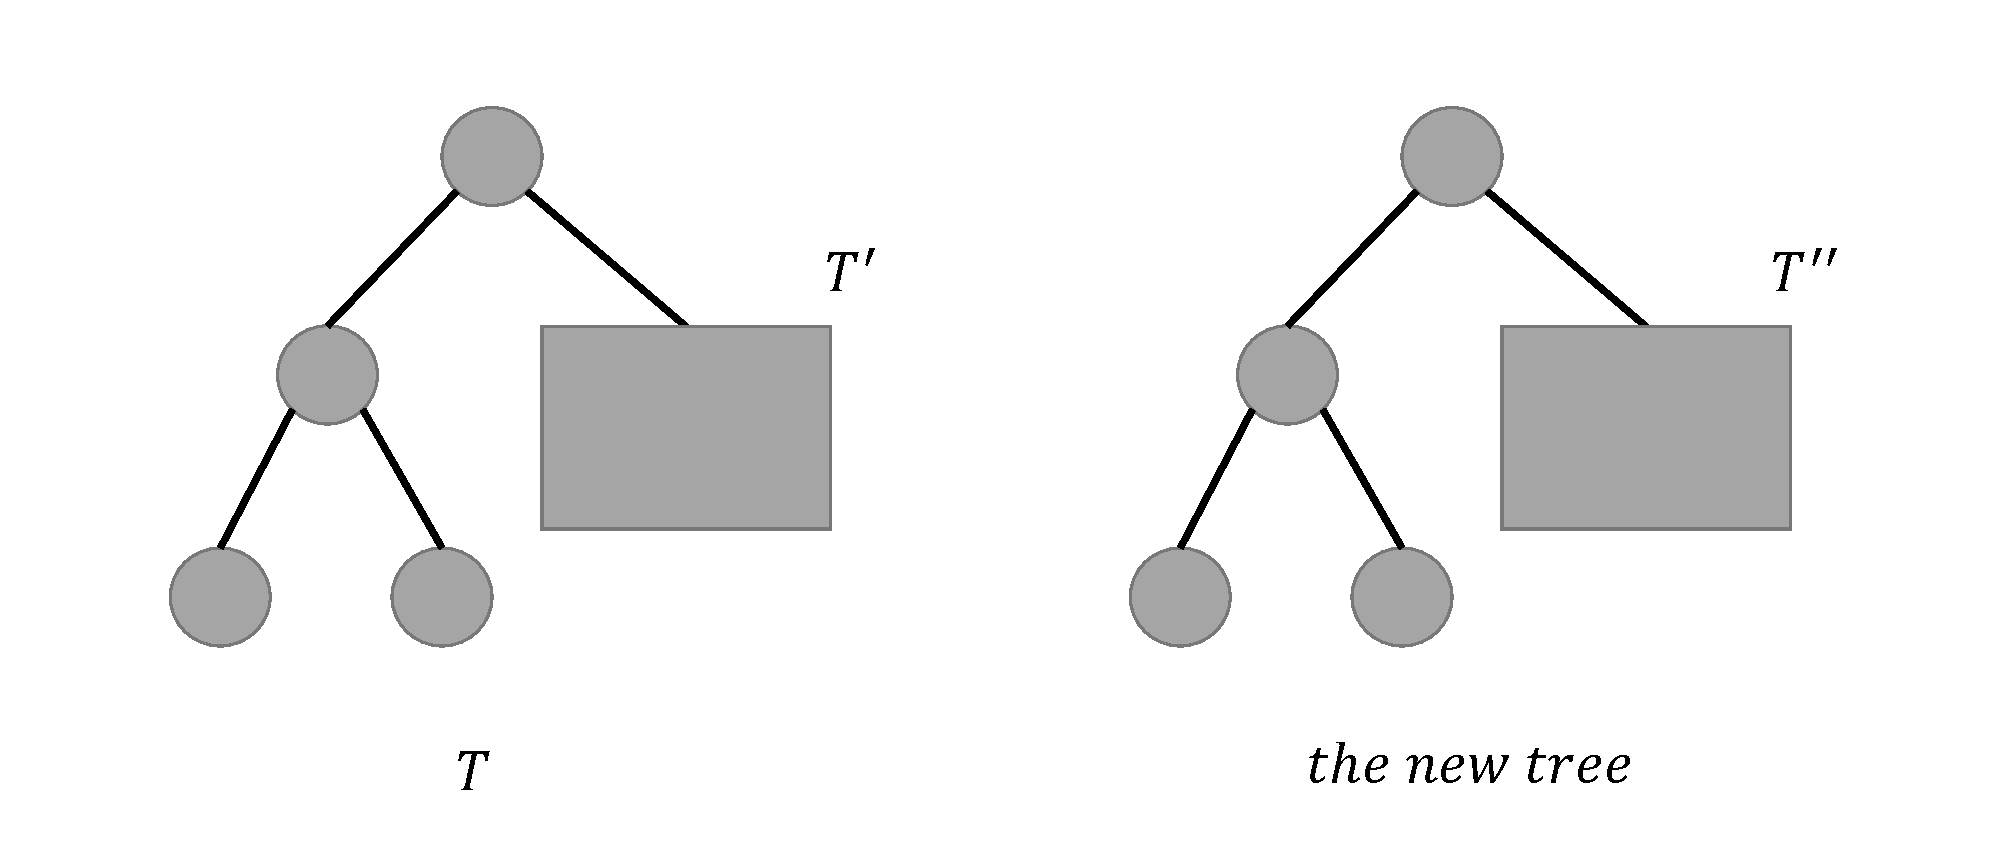
\includegraphics[width=0.8\textwidth]{Fig-Subtree.pdf}
                \caption{Proof for Optimal Substructure}\label{Fig-Subtree}
            \end{figure}
                \item Now that we have proved the optimal substructure property, we can use it to construct the state transition equation. For an optimal binary search tree containing $k_i,\dots,k_j$, it must be composed of a root node $k_r(i\leq r\leq j)$ and an optimal subtree containing $k_i,\dots_{r-1}$ and another optimal subtree containing $k_{r+1},\dots,k_j$. Then we just need to enumerate $k_r$ to get the whole optimal tree. Note that if $r = i$ or $r = j$, then the left subtree or the right subtree will only contain $d_{i-1}$ or $d_j$.\\
                Then, we'll derive the state transition equation by cases.\\
                \begin{enumerate}[i]
                    \item If $j = r-1$, then $e(i,j) = q_{i-1}$.
                    \item If $j\ge i$, we can find that the expected search cost of the left subtree and right subtree will increase by $w(i,r-1)$ and $w(r+1,j)$ respectively. By enumeration, we get the state transition equation
                    \begin{align*}
                        e[i,j] = min_{i\leq r \leq j}\{p_r+e[i,r-1]+w(i,r-1)+e[r+1,j]+w(r+1,j)\}
                    \end{align*}
                    In fact, we have $w(i,j) = p_r+w(i,r-1)+w(r+1,j)$, then we have
                    \begin{align*}
                        e[i,j] = min_{i\leq r \leq j}\{e[i,r-1]+e[r+1,j]+w(i,j)\}
                    \end{align*}
                \end{enumerate}
                Therefore, we have already derived the state transition equation
                $$
            e[i,j] = \left\{  
             \begin{aligned}
             &q_{i-1},  &j =& i-1 \\  
             &min_{i\leq r \leq j}\{e[i,r-1]+e[r+1,j]+w(i,j)\},  &j\ge& i  
             \end{aligned}  
            \right.  
            $$
            In order to optimise time efficiency, we definitely need to store sub-results. Then two 2-D arrays $e[1\dots n+1,0\dots n]$ and $w[1\dots n+1,0\dots n]$ are both needed. Also, we need $r[1\dots n,1\dots n]$to store the root node of the current tree so that we can draw the tree after we find the final answer.\\
            There still exists one problem——in which order should we compute $e[1\dots n+1,0\dots n]$. A natural idea is to compute intervals with shorter length first.\\
            Thus, we can write the pseudocode (Alg.\ref{tree-dp}).
            \item
            Please refer to \emph{Code-OBST.cpp}. \\ Now let's analyze the time complexity.
            The first loop obviously has a time complexity of $\Theta(n)$. The inner part of the 3-layer loop cost $\Theta(1)$. Thus, the time complexity of the 3-layer loop is
            \begin{align*}
                \begin{split}
                    T(n) &= \sum_{i=1}^{n}\sum_{j=1}^{n-i+1}\sum_{k=j}^{j+i-1} \Theta(1)\\
                    & = \sum_{i=1}^{n}\sum_{j=1}^{n-i+1} \Theta(i)\\
                    & = \sum_{i=1}^{n} \Theta(i(n-i+1)) = \sum_{i=1}^{n} \Theta(in - i^2+i)\\  
                    &= \Theta(\frac{n^2(n+1)}{2}-\frac{n(n+1)(2n+1)}{6}+\frac{n(n+1)}{2}) = \Theta(n^3)
                \end{split}
            \end{align*}
            Thus, the time complexity is $\Theta(n^3)$.\\
            The minimum search cost calculated by the algorithm is 3.12.
            
            \begin{minipage}[t]{0.8\textwidth}
            \begin{algorithm}[H]
            \KwIn{Two arrays of probability $p[1\dots n],q[0\dots n]$}
            \KwOut{Two 2-D arrays $e[1\dots n+1,0\dots n]$ and $r[1\dots n,1\dots n]$, which imply the expected search cost and root of the subtree containing $k_i,\dots,k_j$}
            		
            \BlankLine
            \caption{Find the Optimal Binary Search Tree through Dynamic Programming}
            \label{tree-dp}
            $e[1\dots n+1,0\dots n]\leftarrow [0\dots 0,0\dots 0]$\;
            $w[1\dots n+1,0\dots n]\leftarrow [0\dots 0,0\dots 0]$\;
            $r[1\dots n,1\dots n]\leftarrow [0\dots 0,0\dots 0]$\;
            \For{$i = 1 \text{ to } n+1$ }{
                $e[i,i-1] = q_{i-1}$\;
                $w[i,i-1] = q_{i-1}$\;
            }
            \For{$len = 1 \text{ to } n$ }{
                \For{$i = 1 \text{ to } n-len+1$ }{
                    $j = i+len-1$\;
                    $w[i,j] = w[i,j-1]+p_j+q_j$\;
                    $e[i,j] = \infty$\;
                    \For{$root = i \text{ to } j$ }{
                        $temp = w[i,j]+e[i,root-1]+e[root+1,j]$\;
                        \If{temp<e[i,j]}{
                            $e[i,j]=temp$\;
                            $r[i,j]=root$\;
                        }
                    }
                }
            }
            \Return $e$ and $r$\;
            \end{algorithm}
            \end{minipage}
            
            \item
            Because we have already recorded the root of  every optimal subtree, we can just do a preorder traversal through the tree. We start with $r[1][n]$, and for each time, we can find a new root $r[i][j]$ and divide the original tree into two subtrees. We repeat these steps until $r[i][j] = i$ or $r[i][j] = j$, which mean we arrive the lowest internal nodes and we can just add ``leaves''($d_{i-1}$ or $d_{j}$) to it.
            \begin{figure}[htbp]
                \centering 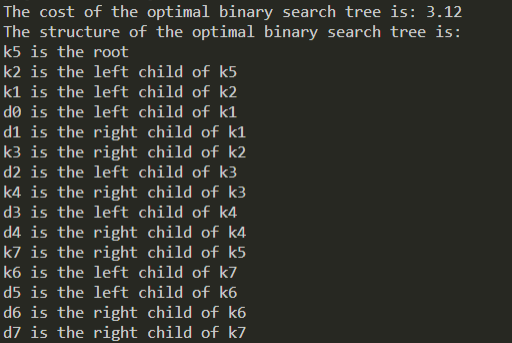
\includegraphics[width=0.5\textwidth]{Fig-TreeResult.png}
                \caption{Structure of OBST Generated by the Program}\label{Fig-TreeResult}
            \end{figure}
    		Then, we can draw the structure of the OBST.
    		\begin{figure}[htbp]
                \centering 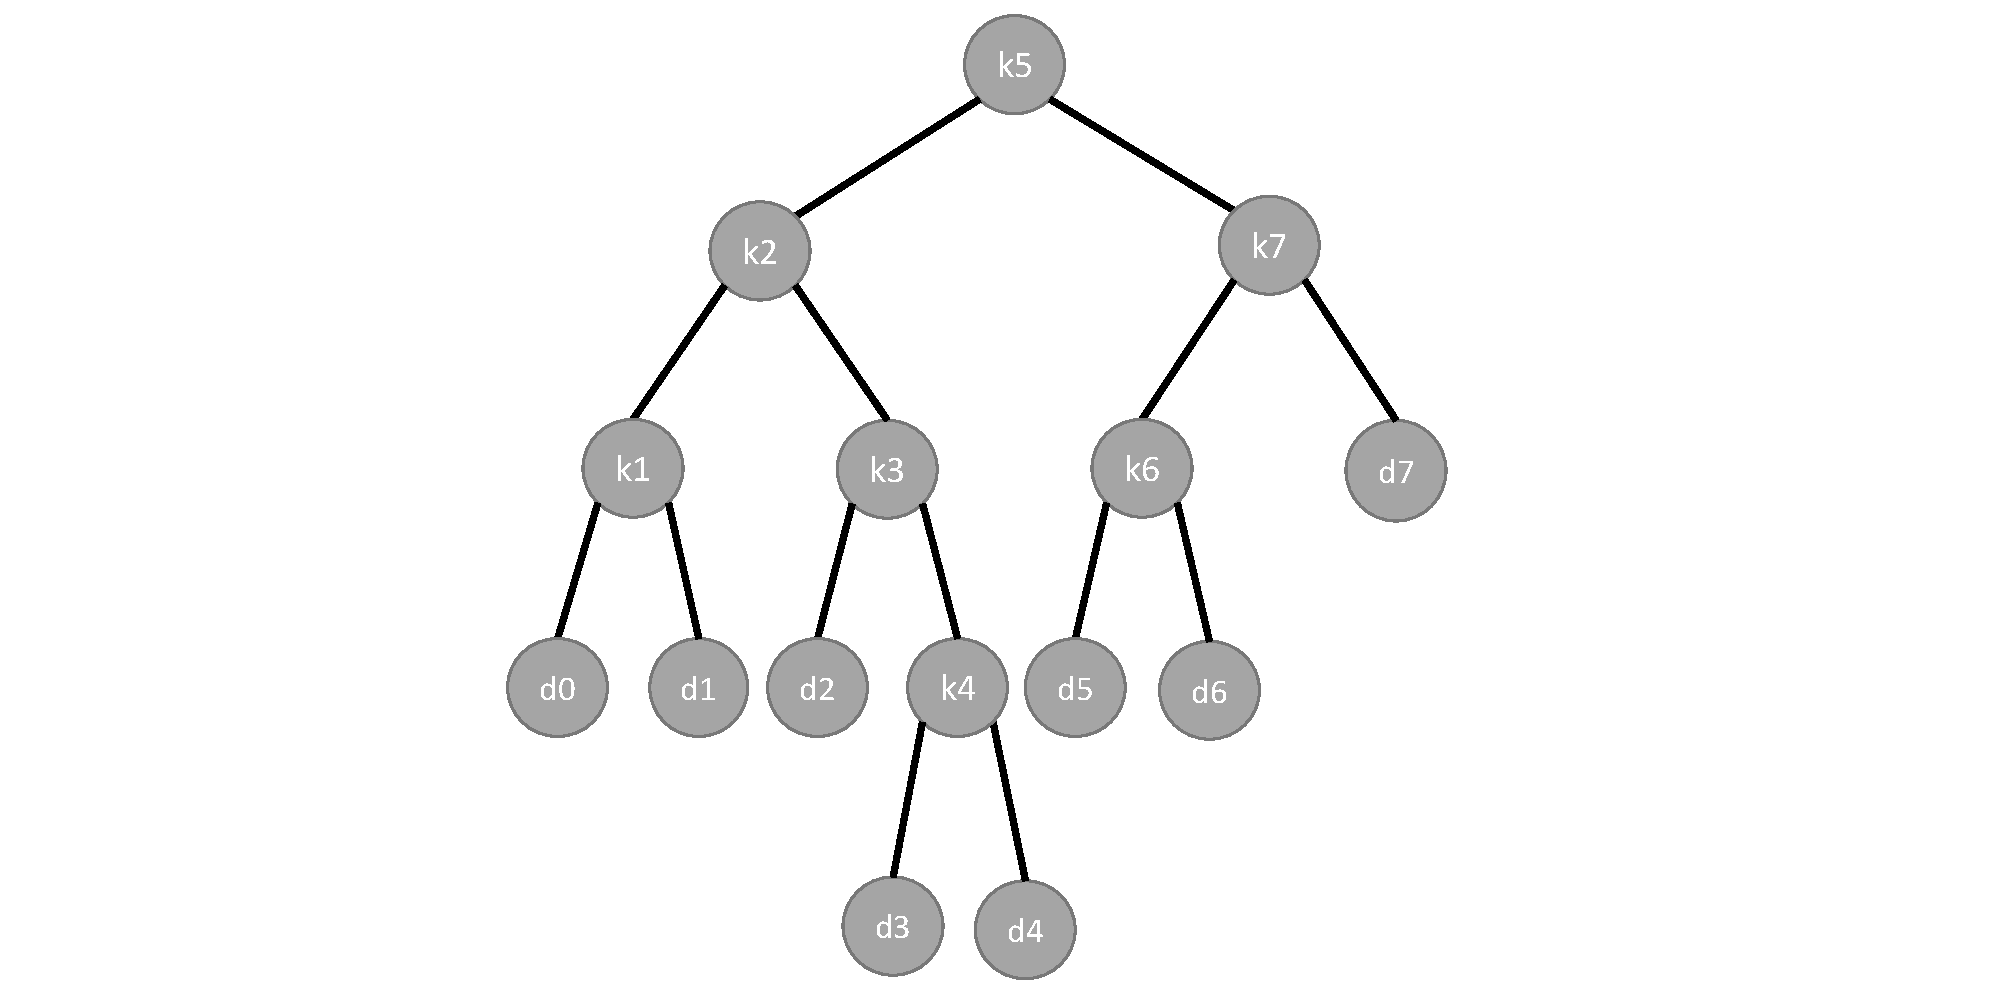
\includegraphics[width=0.9\textwidth]{Fig-OBST.pdf}
                \caption{Structure of OBST}\label{Fig-OBST}
            \end{figure}
    		\end{enumerate}
		\end{solution}
		
		\item \textit{Dynamic Time Warping Distance.} \textbf{DTW} stretches the series along the time axis in a dynamic way over different
		portions to enable more effective matching. Let $D T W(i, j)$ be the optimal distance between the first $i$ and first $j$ elements of two time series $\bar{X}=\left(x_{1} \ldots x_{n}\right)$ and $\bar{Y}=\left(y_{1} \ldots y_{m}\right),$ respectively. Note that the two time series are of lengths $n$ and $m$, which may not be the same. Then, the value of $D T W(i, j)$ is defined recursively as follows:
		$$
		DTW(i, j)=\left|x_{i}- y_{j}\right|+\min(DTW(i, j-1), DTW(i-1, j), DTW(i-1, j-1))
		$$
		
		\begin{enumerate}
			\item Implement the proposed DTW algorithm in C/C++ and analyze the time complexity of your implementation. ({\color{blue}The framework Code-DTW.cpp is attached on the course webpage}). Two test cases have been given in the source code. 
			\item The window constraint imposes a minimum level $w$ of positional alignment between matched elements. The window constraint requires that $DTW(i, j)$ be computed only when $|i-j| \leq w$. Modify your code to add a window constraint and give the results of $ w=0 $ and $ w=1 $ on the two test cases. 
		\end{enumerate}
		\begin{solution}
		~
		\begin{enumerate}
		    \item Please refer to \emph{Code-DTW.cpp}.\\
		    The result are shown as below.
		    \begin{figure}[htbp]
                \centering 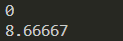
\includegraphics[width=0.3\textwidth]{Fig-DTWResult.png}
                \caption{DTW Result Without Window Constraint}\label{Fig-DTW}
            \end{figure}

		    Let us analyze the time complexity. In fact, for the whole process of filling the cost matrix, we have a 2-layer loop, which has a time complexity of $\Theta(nm)$. For the process of generating the warping path, the time complexity is $O(n+m)$. Thus, the time complexity is $\Theta(nm)$.
		    \item Please refer to \emph{Code-DTW.cpp}.\\
		    To implement constraint window, we can check every time we access or revise $DTW[i][j]$. The running result are shown in Figure \ref{Fig-DTWConstraint}.
		    
		    \begin{figure}
            \centering
            \subfigure[w = 0]{
            \label{Fig-w0}
            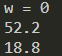
\includegraphics[width=1in]{Fig-DTW-w0.png}}
            \hspace{1in}
            \subfigure[w = 1]{
            \label{Fig-w1}
            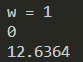
\includegraphics[width=1.2in]{Fig-DTW-w1.png}}
            \caption{DTW Result With Window Constraint}
            \label{Fig-DTWConstraint} 
            \end{figure}
            
		\end{enumerate}
		\end{solution}
		
	\end{enumerate}
	
	\vspace{20pt}
	
	\textbf{Remark:} You need to include your .pdf and .tex and {\color{red}\emph{$2$}} source code files in your uploaded .rar or .zip file. Screenshots of test case results are acceptable.
	
	%========================================================================
\end{document}
